\section{Introduction}
\label{sec:HomographyIntroduction}

This section is dedicated to one of our experiments that were not completely related to the \gls{vot} itself, yet we achieved an original scientific contribution in this area when exploring certain solutions that could potentially be applicable to object tracking, especially traffic analysis. Even though we did not set out for homography-based object tracking (explained later) due to limitations of available datasets, still we would like to elaborate on our developed approach. The proposed method was fully described as well as scrupulously tested under difficult conditions. We wrote up the whole research process in a paper called \textbf{Homography Ranking Based on Multiple Groups of Point Correspondences}~\cite{ondrasovic2021homography}, published in journal \textbf{Sensors} (web:~\cite{sensors}), under the category \emph{Physical Sensors}. In what follows, we provide a concise report of our research. For more information, we suggest the reader use the aforementioned article, even though a great deal of information is duplicated here. Moreover, our preliminary discussion of this possibility with initial proposal of the solution can be found in our first paper dubbed \textbf{Foundations for homography estimation in presence of redundant point correspondencies}~\cite{ondravsovivc2020foundations} published in \textbf{Mathematics in Science and Technologies} (web:~\cite{mistconf}) conference.

\section{Motivation}
\label{sec:HomographyMotivation}

One of the fundamental tasks of computer vision is to deal with various image transformations that may improve the outcome of subsequent post-processing phase. One transformation that was of particular interest to our goal of traffic analyis is the perspective transformation. More concretely, a removal of perspective distortion. To achieve this, the so-called homography mapping is often exploited.

Homography is a perspective projection of a plane from one camera view into a different camera view. The perspective projection maps points from a $3$D world onto a $2$D image plane along lines that emanate from a single point~\cite{geetha2013automatic, bousaid2020perspective}. This projection is performed by a $3 \times 3$ invertible transformation matrix called the homography matrix (or just homography) with $8$ \gls{dof}. A general homography matrix may be defined as
\begin{equation}
    \label{eq:HomographyMatrix}
    \H =
    \begin{bmatrix}
        h_{11} & h_{12} & h_{13}\\
        h_{21} & h_{22} & h_{23}\\
        h_{31} & h_{32} & h_{33}
    \end{bmatrix}
\end{equation}
This transformation is used to achieve a mapping between two views of the same plane, since in the pinhole camera model any two images of the same planar surface are related to each other by the homography~\cite{hartley2003multiple, hartley1997defense}. More specifically, a single vector $\vectt{u}{u_x, u_y, 1}$, representing a warped keypoint in homogeneous coordinates, is mapped onto the rectified keypoint  $\vectt{\tilde{u}}{\tilde{u}_x, \tilde{u}_y, 1}$ by the homography $\H$ using the transformation $s \vect{\tilde{u}} \approx \H \vect{u}$, with $s$ being the scale factor. In its most general form, homography may achieve mapping between various perspectives. However, for our purposes, we focused only on producing a view where perspective distortion is absent, i.e., to rectify the image so that it looks as if the camera was in an orthogonal position with respect to the desired plane in the world when taking the picture.

Homography is commonly used for rectification of text document images by generating a fronto-parallel view~\cite{lu2005perspective, miao2006perspective}, image stitching~\cite{adel2014image, gao2011constructing}, video stabilization~\cite{liu2015smooth}, extracting metric information from $2$D images~\cite{zhang2000flexible}, pose estimation~\cite{circularmarkerposeestim}, and for various traffic-related applications, e.g., ground-plane detection~\cite{arrospide2010homography}, and bird's-eye view projection~\cite{luo2010low}.

The primary motivation to explore the possibility of employing homography for \gls{vot} was the fact that as long as a static camera is used and few assumptions that we will discuss later hold, the scene may be easily stripped off the effect of the perspective distoriton. Considering this, the incentive to track vehicles visually using a static camera while exploiting a fronto-parallel view over the road seemed like a plausible extension with possible advantages for traffic analysis. Furthermore, the combination of homography and object tracking is present in the literature, e.g.~\cite{Bose04groundplane, Zhang2012, Mei2009}. To provide more detail, Bose et al.~\cite{Bose04groundplane} presented a fully automated technique for both affine and metric rectification of a given ground plane (up to a scale factor) by simply tracking moving objects. The derivation of the necessary constraints for projective transformation between the image and the ground plane was obtained by observing objects that moved at constant velocity in the world for some part of their trajectory. We conjectured that the extra information about the scene geometry that we may achieve using rectification could aid in making the tracking more accurate. Visual trackers are often supported by motion models such as Kalman filter~\cite{Kalman1960}, so the rationale was to estimate motion model in a orthogonal projection, rather than perspectively distorted one.

\begin{figure}[t]
    \centerline{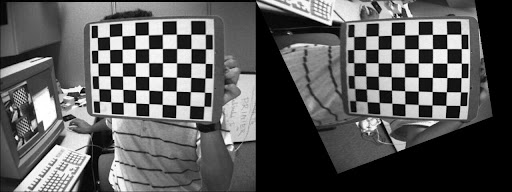
\includegraphics[width=\linewidth]{figures/homography/chessboard_marker.jpg}}
    \caption[Chessboard marker]{An example of a chessboard marker present in a scene that may be used to establish a point correspondence that would serve for a homography transformation. The rectified, fronto-parallel view demonstrates a desired effect that points present on the ``ground'' plane (in this case, the chessboard) are properly projected, whereas other points suffer from substantial distortion. \externalsrc{\cite{homographybasicscode}}}
    \label{fig:ChessboardMarker}
\end{figure}

\begin{figure}[t]
    \centerline{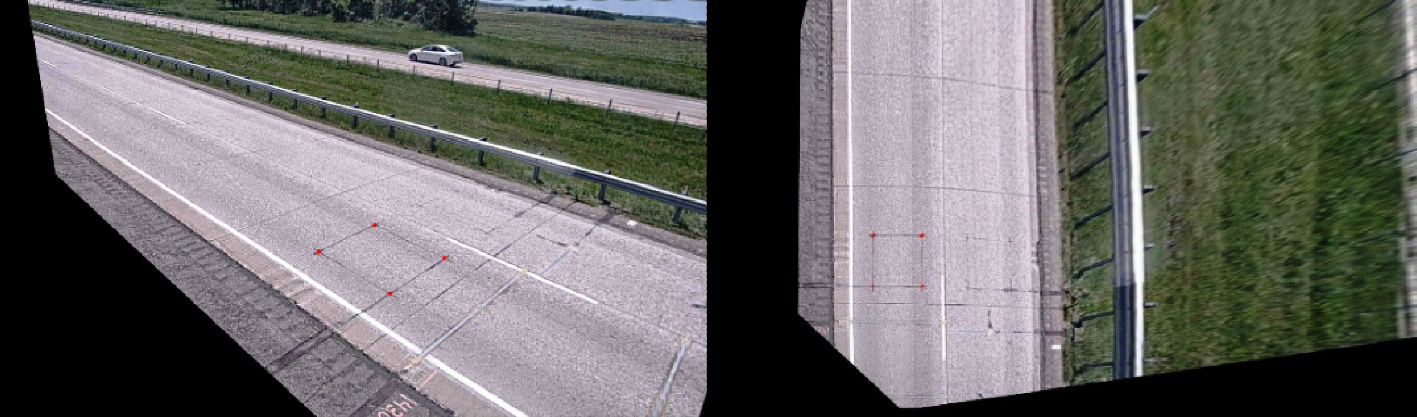
\includegraphics[width=\linewidth]{figures/homography/homography_road.png}}
    \caption[Square marker on a road]{An example of a virtual square marker present on a road that may be used to establish a point correspondence, and thus the homography transformation, too. The obtained view allows for many applications such as speed and size measurements that would otherwise be a lot more problematic in a perspectively deformed view. \externalsrc{\cite{Bose04groundplane}}}
    \label{fig:RoadMarker}
\end{figure}

A common approach to estimate the homography is to use a set of at least four $2$D point correspondences~\cite{hartley1997defense}. We refer to the points used for establishing the $2$D point correspondences as keypoints. These keypoints may belong to a marker which is an object with a known shape that is either naturally occurring or artificially positioned in the scene. A regular pattern like a chessboard is usually utilized~\cite{zhang2016flexible} (see Fig.~\ref{fig:ChessboardMarker}). A single marker is identified in the image by multiple independent keypoints that have a direct correspondence to its real shape, thus making a group of point correspondences. For the sakes of traffic analysis, the marker may be represented by virtually any points on the image as long as certain conditions are met (see Fig.~\ref{fig:RoadMarker}). However, point correspondences established this way are often noisy and they can introduce errors in the homography estimation. Although $4$ keypoints are satisfactory, often a greater number of keypoints is used, allowing to use optimization to minimize a suitable cost function~\cite{osuna2016multiobjective, mou2013robust}. Then, outlier removal becomes an important step, and algorithms such as RANSAC~\cite{fischler1981random} are usually employed.

\begin{figure}[t]
    \centerline{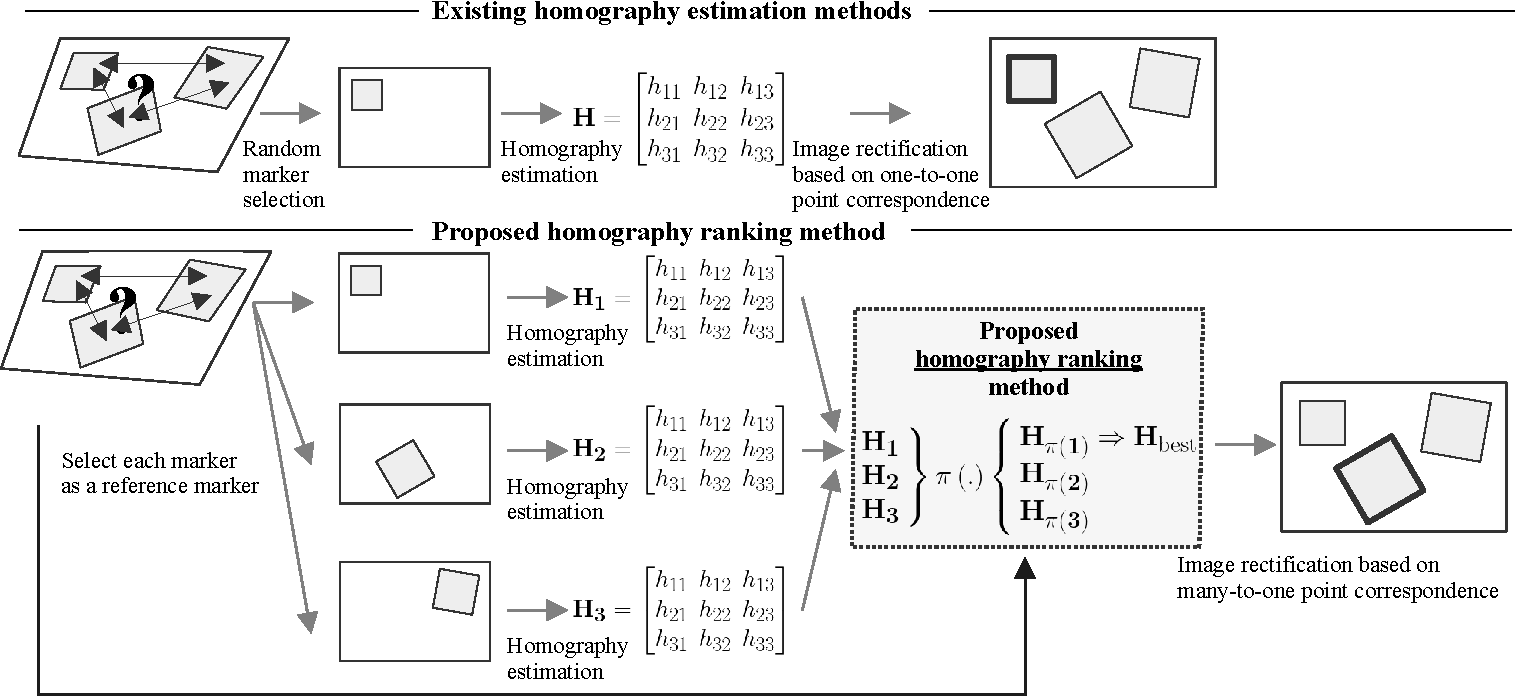
\includegraphics[width=\linewidth]{figures/homography/motivation_diagram.pdf}}
    \caption[Homography ranking motivation diagram]{Difference between existing homography estimation methods and the proposed homography ranking method. In presence of multiple markers without information about their relative positions in the world, existing approaches can only estimate isolated homographies without the ability to select the best one. Our method extends existing approaches by exploiting multiple markers to rank the isolated homographies.}
    \label{fig:HomographyMotivationDiagram}
\end{figure}

This work was motivated by a real-world application of generating a bird's-eye view over a road (see Fig.~\ref{fig:RoadRectification}) from a video recording when we could not use a large marker to cover a sufficient portion of the road (see Fig.~\ref{fig:MultipleMarkersOnRoad}). Homography estimation based on a single small marker was inaccurate. Therefore, we tried to use multiple small markers and measure their relative positions. However, their position measurements were highly noisy at best. Thus, the proposed method was used, instead. It is important to note that our method can also be adopted in a situation when the marker placed at various positions on the same planar surface is visible at different frames using a static camera. Stacking the frames onto each other yields a view with multiple markers.

Let us now describe the underlying incentive for developing our approach. Assume a presence of a sole marker in the scene (Fig.~\ref{fig:RoadMarker}). Even though the marker is distorted under perspective, the knowledge of its real shape makes it possible to compute the homography. When multiple copies of the same marker are visible, but their positions in the world are unknown, the knowledge of the shape is not enough to incorporate all the keypoints in the estimation. In the absence of position information, existing approaches for homography estimation based on point correspondences fail because the projection has to preserve the proportional positions. Thus, estimating the homography without knowing the ground-truth layout of the keypoints up to an arbitrary scale does not guarantee the correct result.

Under the aforementioned constraints, existing methods can only generate an isolated homography for each marker based on the one-to-one point correspondence (see Fig.~\ref{fig:HomographyMotivationDiagram}). Each homography may be affected by different sources of noise, e.g., low resolution, blur, or keypoint detection. Thus, the outcome of rectification may vary. Additionally, in many practical applications, a single marker usually covers a small portion of the image which increases susceptibility to noise. The trivial solution would be to use a bigger marker that covers the majority of the estimated plane in the image. However, this solution is often impractical. Furthermore, it is not possible to simply ``merge'' multiple isolated homographies together.

\begin{figure}[t]
    \centerline{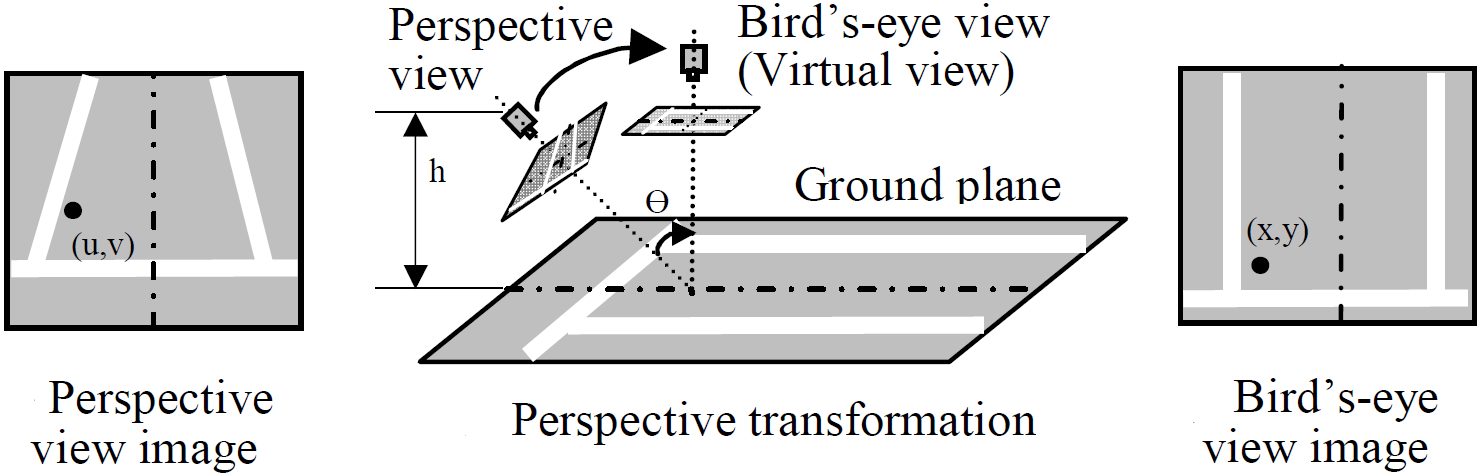
\includegraphics[width=0.8\linewidth]{figures/homography/road_rectification.png}}
    \caption[Road rectification]{A demonstration of the rectification process when obtaining a fronto-parallel view over the road using homography. \externalsrc{\cite{Luo2010}}}
    \label{fig:RoadRectification}
\end{figure}

\begin{figure}[t]
    \centerline{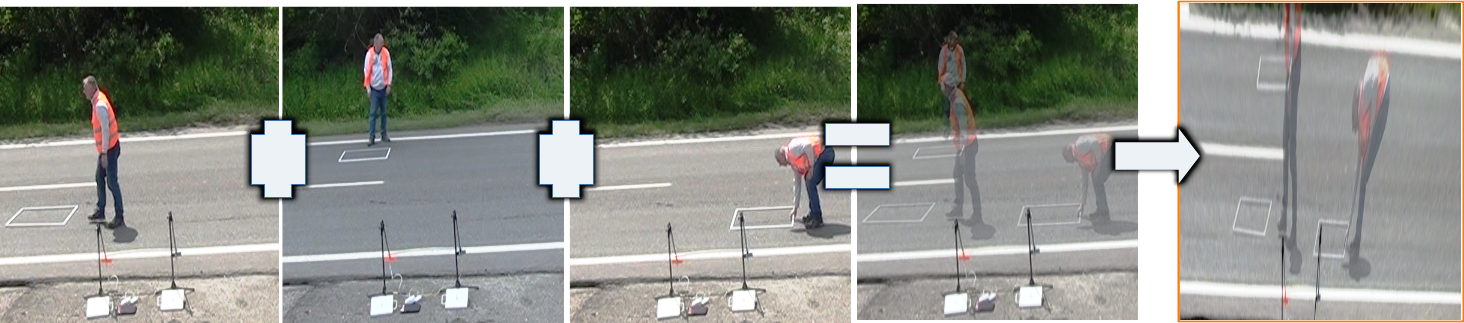
\includegraphics[width=\linewidth]{figures/homography/markers_on_the_road.png}}
    \caption[Multiple markers on the road]{A motivating real-world example for the proposed method. We can see different frames captured during a video recording that show various positions of the same marker. The picture after the ``equality'' sign is a merge of the previous frames for better illustration. Due to the use of a static camera, we may treat positions of the given marker on individual frames as if they were captured simultaneously. However, the question still remains unanswered. Given multiple markers in the absence of their position information, which one is the best to choose for rectification?}
    \label{fig:MultipleMarkersOnRoad}
\end{figure}

\section{Preliminaries}
\label{sec:HomographyPreliminaries}

In this section, we describe our established terminology. Even though there are standard conventions for naming certain aspects of our problem, we nevertheless had to invent few more terms to ease information delivery and improve clarity.

A~marker is an object with a known, easy-to-detect shape. This object is either naturally occurring or artificially placed on the planar surface of the scene we want to produce a bird's-eye view for, i.e., to remove perspective distortion. The marker contains keypoints, a set of distinct, independent, visual feature points, e.g., corners. The chosen keypoints visible in the perspectively deformed image are called the \mbox{warped keypoints}. The set of the \mbox{rectified keypoints} in the desired image (not subjected to perspective distortion) is produced from the warped keypoints using the homography projection. The \mbox{point correspondence} is a relationship between the warped and the \mbox{target keypoints} and it is used for homography estimation. Ideally, the rectified keypoints match the target keypoints. See Figure~\ref{fig:HomographyTerminology} for details.

\begin{figure}[t]
    \centering
    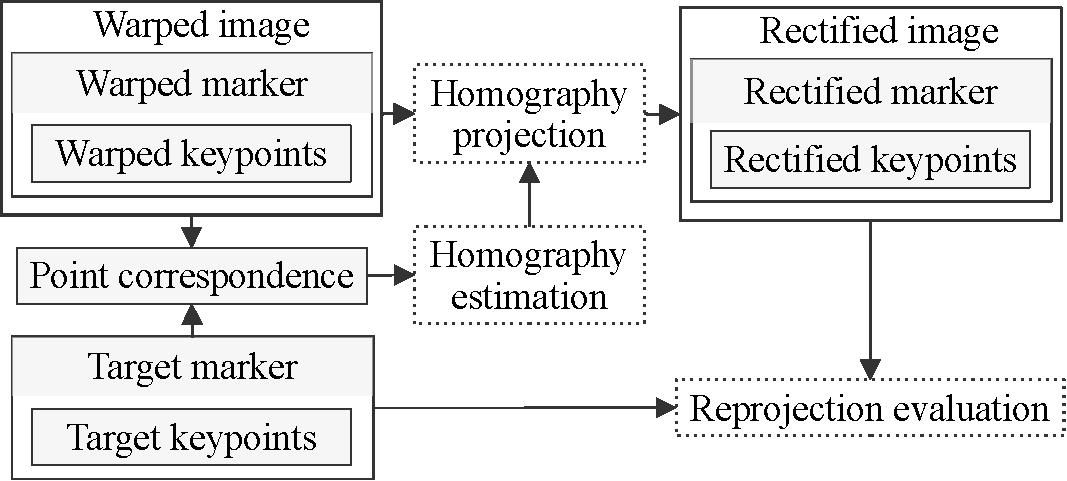
\includegraphics[width=0.6\linewidth]{figures/homography/terminology.pdf}
    \caption{Visualization of relationships in our established terminology. The diagram also shows the hierarchical dependence of individual terms. Dotted elements represent processes with arrows denoting their input and output.}
    \label{fig:HomographyTerminology}
\end{figure}

Without stating otherwise, a \mbox{\textbf{similarity transformation}} will denote a limited affine transformation with $4$ DoF consisting of translation, rotation and uniform scaling (equation \eqref{eq:SimilarityMatrices}). Let $\mset{K}_1$ and $\mset{K}_2$ be sets of feature keypoints belonging to objects $O_1$ and $O_2$. We say that objects $O_1$ and $O_2$ are \mbox{\textbf{similar}} if there exists a similarity transformation $\psi$, such that $\mset{K}_1 = \func{\psi}{\mset{K}_2}$ and $\mset{K}_2 = \func{\psi^{-1}}{\mset{K}_1}$. For example, $O_1$ and $O_2$ may be rectangles of different sizes but with an identical aspect ratio.

Let $m$ be the number of markers and $k$ be the number of keypoints of each marker. Each $i$-th marker is described by a $3 \times k$ matrix $\suprbrackets{\mtx{W}}{i}$ containing its warped keypoints as

\begin{equation}
    \suprbrackets{\mtx{W}}{i} =
    \begin{bmatrix}
        \supsubrbrackets{x}{1}{i} & \supsubrbrackets{x}{2}{i} & \dots & \supsubrbrackets{x}{k}{i}\\
        \supsubrbrackets{y}{1}{i} & \supsubrbrackets{y}{2}{i} & \dots & \supsubrbrackets{y}{k}{i}\\
        1                         & 1                         & \dots & 1
    \end{bmatrix},
    i = 1, \dots, m.
\end{equation}

\noindent The target keypoints are specified analogically by the $3 \times k$ matrix $\mtx{T}$. Only one specification is sufficient due to many-to-one correspondence. The ordering of keypoints needs to match the warped keypoints defined above. Thus,

\begin{equation}
    \mtx{T} =
    \begin{bmatrix}
        \tilde{x}_1 & \tilde{x}_2 & \dots & \tilde{x}_k\\
        \tilde{y}_1 & \tilde{y}_2 & \dots & \tilde{y}_k\\
        1           & 1           & \dots & 1
    \end{bmatrix},
\end{equation}

\noindent with the point correspondence being

\begin{equation}
    \supsubrbrackets{x}{j}{i} \simeq \tilde{x}_j, \supsubrbrackets{y}{j}{i} \simeq \tilde{y}_j, i = 1, \dots, m, j = 1, \dots, k.
\end{equation}

\section{Developed Method}
\label{sec:HomographyDevelopedMethod}

The goal of our work was to offer a systematic way to select the ``best'' homography according to the proposed score function without any other prior knowledge about the quality of individual markers.

The method works like this. Each homography is induced by one independent marker. The input to our method is multiple sets (groups) of point correspondences between the warped and the ground-truth markers. So each set represents a marker. Our method can rank multiple homographies and select the best performing one according to the tailor-made score function. Thus, we require a homography matrix for each marker (a set of point correspondences). To compute these matrices, any state-of-the-art method can be utilized. The advantage of our method is that it can rank the referred homographies without the knowledge of absolute or relative positions of markers in the world. We did not propose any method to simultaneously estimate multiple homographies. We build upon the existing homography matrices.

Since we assume no knowledge about the arrangement of markers in the scene, we cannot virtually create one compound marker consisting of all the keypoints. If we could, then we would employ RANSAC or any other sophisticated algorithm to select the best subset of keypoints to estimate the homography. Our approach would be useless. But we only have information about the relative position of marker’s keypoints, not markers themselves. The point correspondence is globally indeterminate. We can only establish a local point correspondence between a single marker and its ground-truth shape. To obtain the isolated homographies, we suggest the user chooses the best method available. 

The homography estimation between existing point correspondences is a standard problem and we heavily rely on its solutions. But we did not contribute to it in terms of improving the homography estimation itself. We provided a way to rank the resulting homographies according to our score function. We developed a way to,
under certain circumstances, choose the ``best'' homography from multiple existing ones. Therefore, our method could not even be compared to RANSAC, because we tackle a different problem.

The proposed method is based on the following assumptions:
\begin{enumerate}
    \item The markers are geometrically similar, i.e., they differ only in translation, rotation, and uniform scale in the real world.
    \item The shape of at least one of them is known.
    \item These markers are placed on the same planar surface in the scene.
\end{enumerate}
Our approach shows a way to relate all the markers to each other in a single score function without knowing their relative positions in the scene. Our method only handles transformation from a distorted to the undistorted view of the target plane. Thus, it serves for the removal of perspective distortion only.

We exploited the properties of homography and similarity transformations and expressed them in a single score function. This function stands at the core of our contribution. Its value is used as a proxy to rank homographies according to their reprojection error over the entire image using only markers' keypoints. The usual use case would be to select the homography with the lowest score, i.e., the highest-ranked matrix, to perform the image rectification.

\begin{figure}[t]
    \centerline{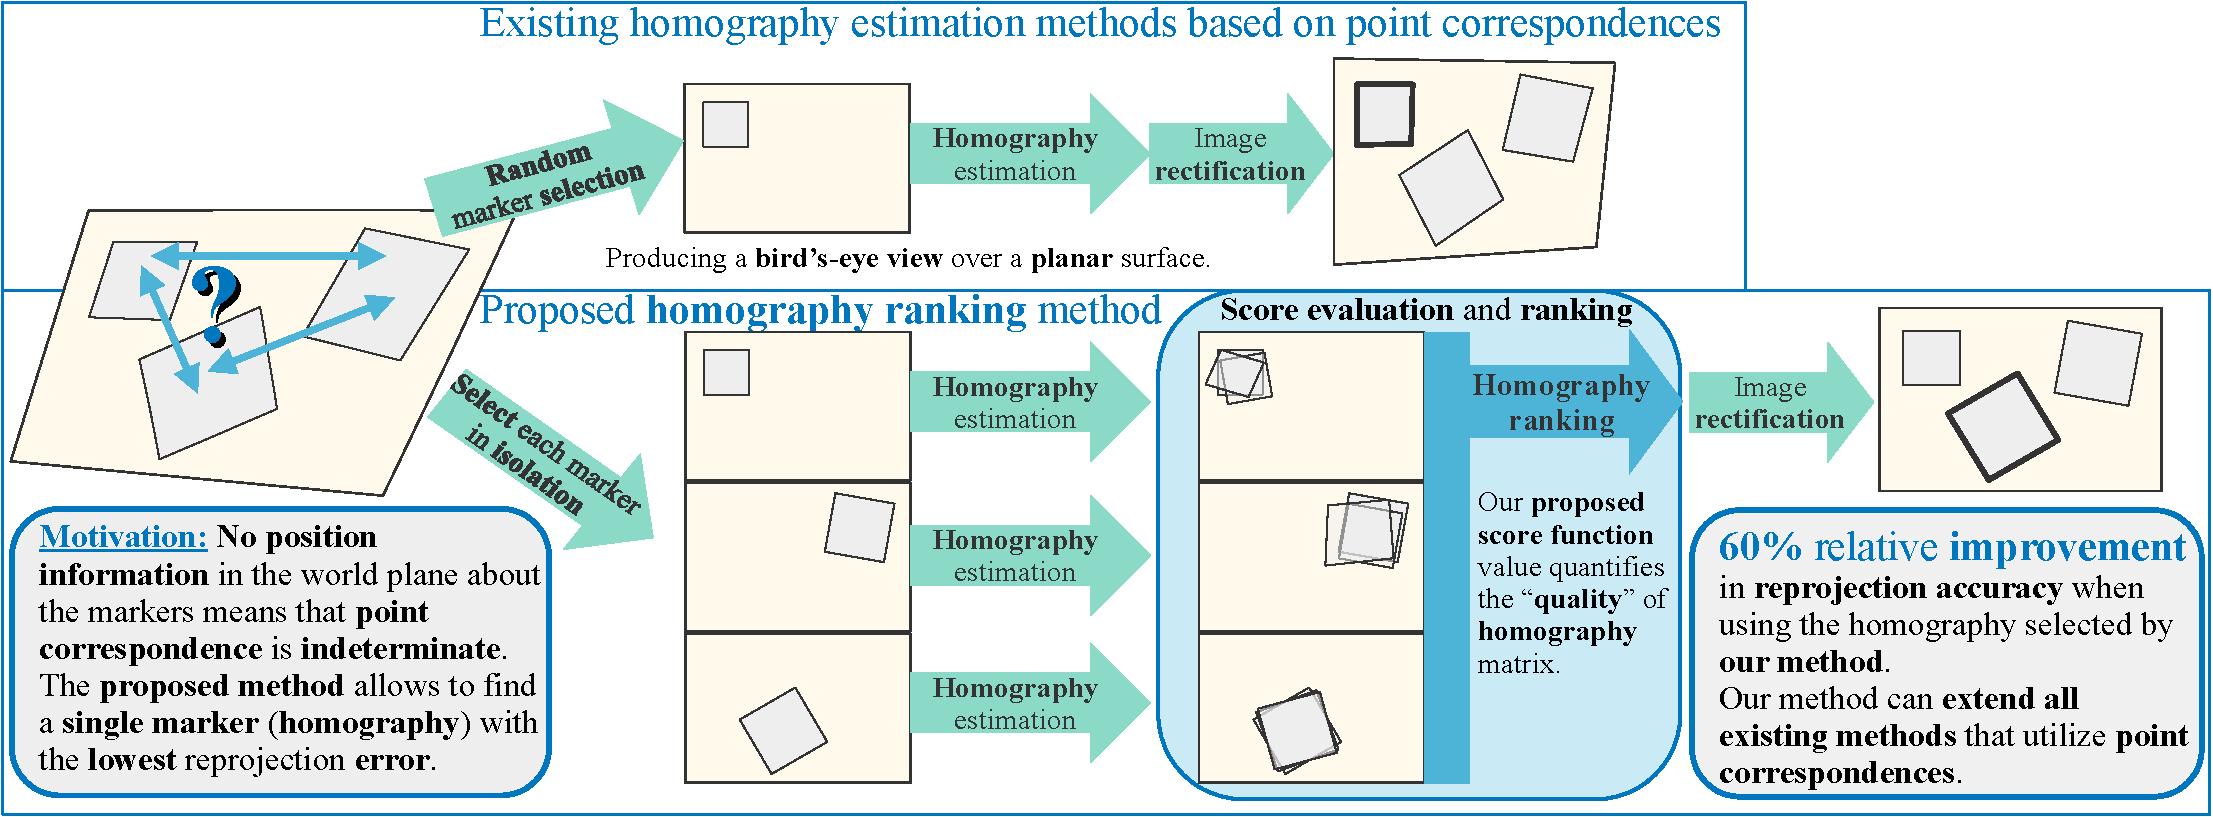
\includegraphics[width=\linewidth]{figures/homography/graphical_abstract.pdf}}
    \caption[Homography ranking graphical abstract]{Here we present the graphical abstract from our paper. The basic idea is that existing approaches may only estimate an isolated homography for each marker and cannot determine which homography achieves the best reprojection over the entire image. Therefore, we proposed a method to rank isolated homographies obtained from multiple distinct markers to select the best homography. This method extends existing approaches in the post-processing stage, provided that the point correspondences are available and the markers differ only by similarity transformation after rectification. We demonstrated the robustness of our method using a synthetic dataset and showed an approximately $60\%$ relative improvement over the random selection strategy based on the homography estimation from the OpenCV library.}
    \label{fig:GraphicalAbstract}
\end{figure}

\begin{figure}[t]
    \centerline{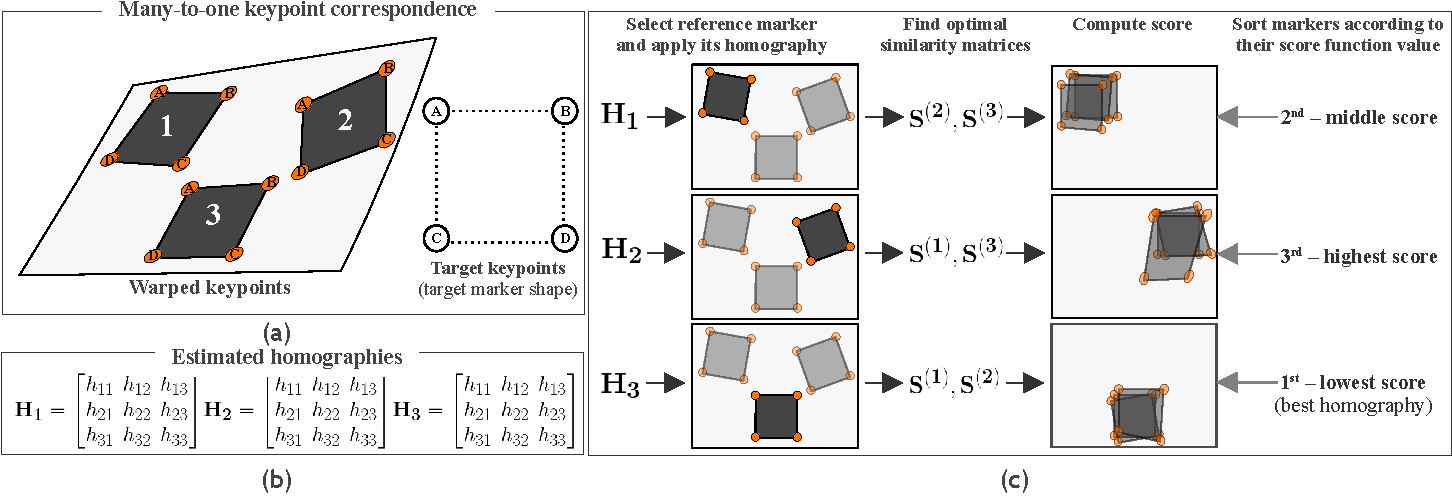
\includegraphics[width=\linewidth]{figures/homography/system_diagram.pdf}}
    \caption[Homography ranking system diagram]{A system diagram describing the general idea behind our method. \textbf{(a)} The input consists of a many-to-one point correspondence specified by geometrically similar markers and information about the shape of the target marker. \textbf{(b)} We assume that the isolated homographies corresponding to each independent marker are provided on the input as well. \textbf{(c)} The algorithm processes each marker by applying its homography matrix to the image to produce a rectified image. Subsequently, it computes optimal similarity matrices corresponding to the auxiliary markers. The computation of the score function makes use of these transformations. The obtained score values then serve for comparison to rank (sort in ascending order) the homographies. The homography ranked first is considered the ``best'' candidate for the minimal reprojection error over the entire image.}
    \label{fig:HomographySystemDiagram}
\end{figure}

Our algorithm is invariant to the underlying homography estimation method. It can thus serve as an extension to approaches that handle point correspondences, either as part of run time or a post-processing stage. Moreover, it is computationally very efficient, as it scales well with a quadratic complexity $\func{\Theta}{m^2}$.

Our method utilizes multiple similar markers (see Figure~\ref{fig:HomographySystemDiagram}). The input is point correspondences and homographies estimated for each marker. Each marker is selected exactly once as a \mbox{reference marker}. All remaining markers are in the role of \mbox{auxiliary markers}. The reference marker's homography is used to perform the perspective transformation to rectify all markers. To rank which reference markers' homography yields the best reprojection, we exploit auxiliary markers. Auxiliary markers are subsequently mapped onto the target marker using similarity transformations (equation~\eqref{eq:SimilarityMatrices}). We then convert the transformed keypoints to homogeneous coordinates and measure the reprojection error as the mean Euclidean distance between the rectified and the target keypoints~\eqref{eq:HomographyScoreFunction}. The aim is to minimize this quantity. The optimal similarity matrices are just auxiliary and redundant after the algorithm ends.

Let $r$ be the index of the reference marker. The $3 \times 3$ matrices describing similarity transformations are contained in a set $\mset{S} = \cbrackets{\suprbrackets{\mtx{S}}{i} \ |\ i = 1, \dots, m}$, such that

\begin{equation}
    \label{eq:SimilarityMatrices}
    \suprbrackets{\mtx{S}}{i} =
    \begin{cases}
        \begin{aligned}
            &\begin{bmatrix}
                1 & 0 & 0\\
                0 & 1 & 0\\
                0 & 0 & 1
            \end{bmatrix} & \text{if } i = r\\
            &\begin{bmatrix}
                \supsubrbrackets{\mtx{R}}{2 \times 2}{i} & \supsubrbrackets{\mtx{T}}{2 \times 1}{i}\\
                \mathbf{0}_{1 \times 2} & 1
            \end{bmatrix} & \text{if }i \neq r\\
        \end{aligned}
    \end{cases},
\end{equation}

\noindent for $i = 1, \dots, m$, where

\begin{equation}
    \supsubrbrackets{\mtx{R}}{2 \times 2}{i} =
    \begin{bmatrix}
        \suprbrackets{s}{i} \cdot \func{\cos}{\suprbrackets{\theta}{i}} & -\suprbrackets{s}{i} \cdot \func{\sin}{\suprbrackets{\theta}{i}}\\
        \suprbrackets{s}{i} \cdot \func{\sin}{\suprbrackets{\theta}{i}} & \suprbrackets{s}{i} \cdot \func{\cos}{\suprbrackets{\theta}{i}}
    \end{bmatrix}, \quad
    \supsubrbrackets{\mtx{T}}{2 \times 1}{i} =
    \begin{bmatrix}
        \supsubrbrackets{t}{x}{i}\\
        \supsubrbrackets{t}{y}{i}
    \end{bmatrix}.
\end{equation}

\noindent This transformation (except for the identity) consists of $4$ DoF: single rotation angle $\suprbrackets{\theta}{i}$, two $x$ and $y$ translation coefficients $\supsubrbrackets{t}{x}{i}$, $\supsubrbrackets{t}{y}{i}$, and a scale coefficient $\suprbrackets{s}{i}$. A full affine transformation with $6$ DoF would be responsible for horizontal and vertical
scales, shear and rotation, and $x$, $y$ offsets~\cite{barath2016novel}. The application of homography that rectifies an image produces a frontal plane which is related to the ground-truth plane by similarity transformation~\cite{hartley2003multiple, beck2016planar}. Thus, we do not include the shear and we only support uniform scaling.

Since all the markers share the same planar surface, any homography has to provide a valid perspective projection, but all perspective projections are subjected to different noise. Our goal is to quantify which homography estimation provides the best perspective projection for the whole plane in the image. To do so, we propose a score function based on the aforementioned constraints. The score function computes a score for individual homographies in conjunction with estimated similarity matrices corresponding to auxiliary markers as

\begin{equation}
    \label{eq:HomographyScoreFunction}
    \func{\scoref}{\H, \mset{S}} =
    \frac{1}{m}
    \sum_{i = 1}^{m}
    \frobnorm{
        \func{h}{
            \suprbrackets{\mtx{S}}{i}
            \H
            \suprbrackets{\mtx{W}}{i}
        }
        -
        \mtx{T}
    },
\end{equation}

\noindent where $\frobnorm{\cdot}$ denotes the Frobenius norm. The function $\func{h}{\cdot}$ converts points to homogeneous coordinates as

\begin{equation}
    \label{eq:HomoCoordsConversion}
    \func{h}{
        \begin{bmatrix}
            x_1 & x_2 & \dots & x_k\\
            y_1 & y_2 & \dots & y_k\\
            z_1 & z_2 & \dots & z_k
        \end{bmatrix}
    } =
    \begin{bmatrix}
        \nicefrac{x_1}{z_1} & \nicefrac{x_2}{z_2} & \dots & \nicefrac{x_k}{z_k}\\
        \nicefrac{y_1}{z_1} & \nicefrac{y_2}{z_2} & \dots & \nicefrac{y_k}{z_k}\\
        1                   & 1                   & \dots & 1
    \end{bmatrix}.
\end{equation}

Now we describe the proposed Algorithm~\ref{alg:HomographyRanking} for homography ranking. Assume a set of warped markers described by warped keypoints and a single target marker described by target keypoints. These objects are linked by a many-to-one point correspondence. Also, assume that homographies have been estimated for each marker in isolation. Our algorithm ascendingly ranks the input set of all pairs $\rbrackets{\suprbrackets{\mtx{W}}{i}, \mtx{T}}$, $i = 1, \dots, m$, by how well each $i$-th marker preserves the target shape of all the markers in the image after removing the perspective distortion. This objective is measured by the score function defined in equation~\eqref{eq:HomographyScoreFunction}. The algorithm evaluates all markers as candidates for the reference marker. In each iteration, it computes optimal similarity matrices for the auxiliary markers in the rectified plane, i.e., after applying the perspective projection induced by the current homography. The aim is to find a homography with a minimal score. The algorithmic complexity is quadratic in the number of markers, thus $\func{\Theta}{m \rbrackets{m - 1} + m \func{\text{log}_2}{m}} \simeq \func{\Theta}{m^2}$.

\def\hmatrices{\boldsymbol{\bar{H}}}
\def\scoref{\mathcal{F}}

\begin{algorithm}[t]
    \caption{Homography Ranking}
    \label{alg:HomographyRanking}
    \begin{algorithmic}[1]
        \State $\hmatrices \gets \arraydef \left[ m \right]$
        \Comment{output array of homographies}
        
        \State $\scores \gets \arraydef \left[ m \right]$
        \Comment{array of scores}
        
        \For{$i \gets 1, \dots , m$}
        
            \State $\hmatrices \left[ i \right] \gets$
            \Call{homography}{$\suprbrackets{\mtx{W}}{i}$, $\mtx{T}$}
            \Comment{retrieve or estimate perspective}
            
            \State $\suprbrackets{\mtx{\bar{S}}}{i} \gets \mtx{I}_{3 \times 3}$
            
            \State $\mset{\bar{S}} \gets \cbrackets{\suprbrackets{\mtx{\bar{S}}}{i}}$
            \Comment{set of similarity matrices}
            
            \ForAll{$j$ : $\cbrackets{1, \dots, m} - \cbrackets{i}$}
            
                \State $\suprbrackets{\mtx{\bar{S}}}{j} \gets$ \Call{similarity}{$\hmatrices \left[ i \right] \cdot \suprbrackets{\mtx{W}}{j}$, $\mtx{T }$}
                
                \State$\mset{\bar{S}} \gets \mset{\bar{S}} \cup \suprbrackets{\mtx{\bar{S}}}{j}$
            \EndFor
            
            \State $\scores \left[ i \right] \gets \func{\scoref}{\hmatrices \left[ i \right], \mset{\bar{S}}}$
            \Comment{evaluate score function \eqref{eq:HomographyScoreFunction}}
        \EndFor
        \State $\sortres \gets \Call{argsort}{\scores}$
        \Comment{indirect sort}
        
        \State \Return $\hmatrices, \sortres$
    \end{algorithmic}
\end{algorithm}

It is important to note that the two functions used in this pseudocode to compute the homography and similarity matrices stand for arbitrary methods that produce the required transformations.

Our score function \eqref{eq:HomographyScoreFunction} is just a proxy for the reprojection error computed over the whole image. Since we utilize only a small subset of points from the entire image, which may be subjected to noise, the assumption that the ``best'' homography is the one our method ranks as first may not hold in every case. In very few cases, the marker that achieves the lowest score function value does indeed reconstruct the remaining markers the best, but not the overall image. However, our experiments show that our method consistently preserves its performance under various conditions.

\section{Experiments and Discussion}
\label{sec:HomographyExperiments}

Fig.~\ref{fig:HeatmapsBestWorst} shows how the reprojection error varies with respect to the marker position. We can see that the marker position can be deduced by looking at the heatmap representing the pixel-wise reprojection error over the image. The transformation achieves the best accuracy in the marker neighborhood and steadily decreases for more distant pixels. However, not all markers are subjected to the same pattern of error variation. This observation was the core motivation for our solution. We aim to choose the marker that minimizes the pixel-wise reprojection error within the region of the image that is as broad as possible. That is why we evaluate our method by computing the reprojection error over each pixel, not just the keypoints.

\begin{figure}[t]
    \centerline{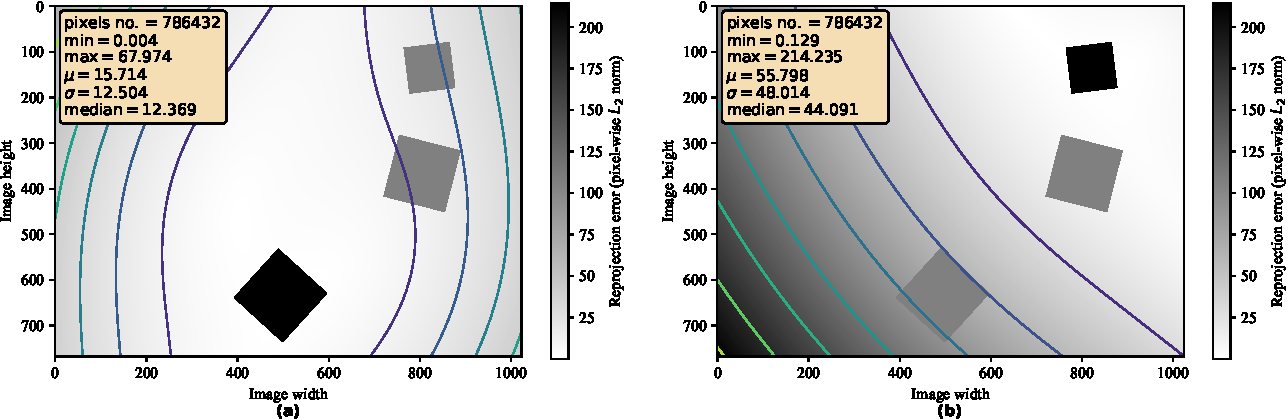
\includegraphics[width=\linewidth]{figures/homography/heatmaps_best_worst.pdf}}
    \caption[Homography ranking heatmaps]{Distribution of pixel-wise reprojection error. The heat map together with corresponding contours demonstrate the varying distance between the ground truth and rectified pixel position after removing the perspective distortion. The bold square represents the reference marker. We show the result of \textbf{(a)} the ``best'' marker and \textbf{(b)} the ``worst'' marker. This test scenario includes all similarity transformations as well as noise in point correspondence.}
    \label{fig:HeatmapsBestWorst}
\end{figure}

We evaluated the proposed homography ranking algorithm in various conditions. We tested cases involving various similarity transformations applied to original markers as well as noisy point correspondence, e.g., errors in marker detection since these are the expected problems in real-world scenarios.

We demonstrated that the proposed solution is robust in presence of noise in the point correspondences. These correspondences can be either algorithmically found using feature-matching algorithms (e.g., SIFT~\cite{lowe1999object}, SURF~\cite{bay2008speeded}) or annotated manually. But even human annotations are often inaccurate. We also showed the robustness of our method to a varying number of markers and a change in shape.

All our test scenarios demonstrated the following trend. On average, the homography with the highest score improved the relative performance to the baseline performance the most (both median and mean above $60$\%). The lowest-ranked homography often led to a lot worse performance (median and mean around $-90$\%). These values varied slightly across different setups. The shape and number of markers had the greatest influence. All the improvements in between steadily decreased, reached $0$\% improvement at around $\nicefrac{2}{3}~m$, where $m$ is the number of markers. A general claim is that the first half of ranked homographies yields a better reprojection compared to the baseline on average. The baseline performance was given by an average OpenCV~\cite{bradski2008learning} reprojection error under the assumption of no prior preference of specific markers, hence the random marker selection.

\subsubsection{Implementation Details}
\label{sssec:HomographyImplementation}

Our proposed algorithm can extend any homography estimation method that exploits point correspondences. For demonstration, we adopted time-tested implementations from the OpenCV~$4.4.0$ library~\cite{bradski2008learning}. Each homography was estimated by the \srcfuncname{findHomography} function which employs DLT~\cite{abdel2015direct} algorithm for $k = 4$ and RANSAC~\cite{fischler1981random} algorithm for $k > 4$, where $k$ is the size of the point correspondences set. Each optimal similarity transformation between two $2$D point sets was estimated by the \srcfuncname{estimateAffinePartial2D}, which also utilizes RANSAC for robustness. We always used default parameters.

\subsection{Dataset Creation}
\label{ssec:HomographyDatasetCreation}

We created a synthetic dataset to simulate the presence of markers in the scene subjected to perspective distortion. Our experiments were based on a pixel-wise comparison of the reprojection error. The synthetic dataset covered multiple setups named as \mbox{\textbf{test scenarios}}. For each test scenario, we generated $t$ different samples to which we refer as \mbox{\textbf{test instances}}. We set $t = 1\ 000$. Table~\ref{tab:TestScenariosResults} contains description of the generated test scenarios. To create test instances (within test scenarios), we employed the procedures described below (see Figure~\ref{fig:DatasetGenerating}).

We organized the creation of our dataset to allow complete reproducibility of the reported results. Thanks to the synthetic nature of our data, fixing the seed for the used pseudo-random generator was sufficient. The source code for running the experiments is freely available (see supplementary materials at the end).

\subsubsection{Image Initialization}
Each test instance was initialized as a blank $1024 \times 768$ image. This image served for $m$ randomly generated copies of the same shape (marker) placed in a $3 \times 3$ grid, where $0 < m \leq 9$. We used a uniform border with $20$\% size of the corresponding side to prevent the generated shapes from reaching outside of the image. We experimented with a different number of markers. From the set of $3 \times 3$ possible anchors, we chose $m$ randomly onto which we placed the generated markers. We also studied the effect of $3$, $5$, $7$, and $9$ out of $9$ possible markers, given that all the similarity transformations and noise were applied. Regarding marker shapes, we tested squares or convex, equilateral polygons, with a tight bounding box of size $100 \times 100$ pixels (covering approximately $1.3$\% of the image). However, other similar shapes could be used, too. Their centroids were evenly distributed over the image whilst the grid cells served as anchors. We adopted random generators from a uniform probability distribution. These settings represented the default configuration. Subsequently, we applied further transformations to the generated markers and the image.

\subsubsection{Similarity Transformation}
We showed the effect of similarity transformations before applying the perspective transformation. The translation and rotation would demonstrate that markers could be positioned arbitrarily in a real environment provided they shared the same planar surface. The change in scale showed that markers could be of different sizes.

To simulate similarity transformation, we applied random rotation from the interval $\left[0, 360\right)$ degrees with origin in the marker center. Then, we generated a random coordinate shift from interval $\sbrackets{-20, 20}$ pixels for translation in $x$ and $y$ direction. However, an identical translation had to be applied to the entire marker to prevent distortion. Then, uniform scaling was performed with the origin in the marker center with a scale factor randomly generated from interval $\sbrackets{0.8, 1.5}$. Due to this range, a ratio of the marker to image area ranged from $1.0$\% to $1.9$\%.

\subsubsection{Perspective Distortion}
We simulated a $3$D rotation of an image around its center to represent a change in perspective on the plane that contained several markers. We rotated the image around its center in $x$, $y$, and $z$ axis by a random angle from interval $\sbrackets{-20, 20}$ degrees to achieve a change in perspective. The original keypoints were transformed along with the entire image, producing the warped keypoints.

\subsubsection{Noisy Point Correspondence}
To simulate a noisy point correspondence, we applied a random noise (translation) to each $x$ and $y$ coordinate of the warped keypoints from the interval $\sbrackets{-2, 2}$ pixels. At this stage, each keypoint was modified in isolation to achieve the distortive effect. Thanks to the perspective deformation, the generated random shift represented different levels of noise depending on how much the image had been warped. This step imitated errors in the marker detection, leading to noisy point correspondence.

\begin{figure}[t]
    \centering
    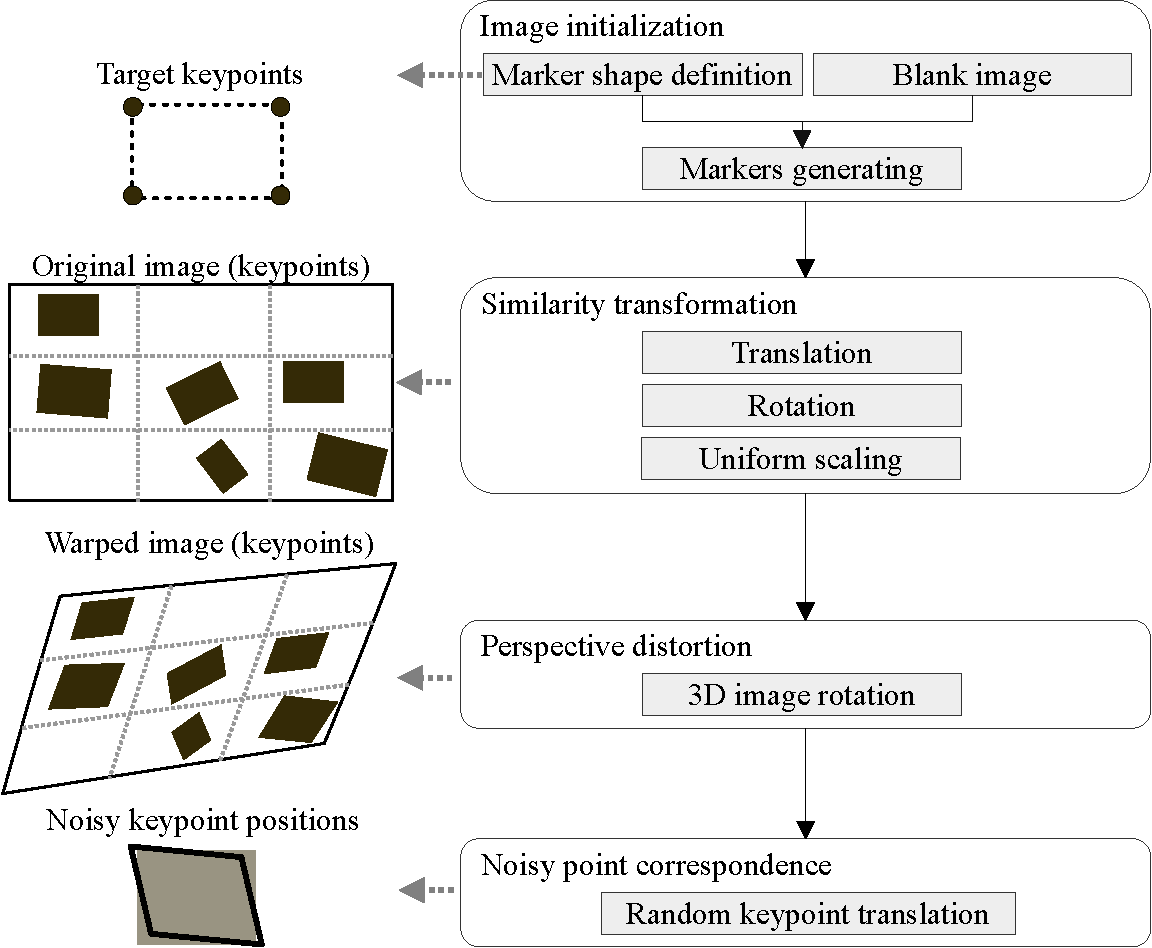
\includegraphics[width=0.7\linewidth]{figures/homography/dataset_generating.pdf}
    \caption{Description of how each one of $t$ test instances in a specific test scenario is created. The input is a blank $w \times h$ image over which $m$ markers are initialized in a uniform grid, which produces the original marker keypoints. Depending on the test scenario, a particular subset of similarity transformations is applied to the entire image. Subsequently, warped keypoints are modified by random noise to simulate noisy point correspondence.}
    \label{fig:DatasetGenerating}
\end{figure}

\subsection{Evaluation Methodology}
\label{ssec:evaluation_methodology}

\subsubsection{Error Computation}
\label{sssec:error_computation}

\def\warpedpix{\vect{w}}
\def\origpix{\vect{g}}

We evaluated the accuracy of our method by measuring the reprojection error using the Euclidean distance between the original and the rectified pixel positions. To obtain an error over the entire image, we computed the error for each pixel. Let $w$ and $h$ be the width and height of the image, respectively. The $3$D rotation of a point in the image around the image center that produces perspective distortion is represented by $\func{\varphi}{\cdot}$. Let $\supsub{\origpix}{i,j}{T} = \sbrackets{j, i, 1}$ be the original (ground-truth) pixel position at the $i$-th row and $j$-th column, and let $\warpedpix_{i, j} = \func{\varphi}{\origpix_{i, j}}$ be the analogically defined warped pixel position, for $i = 1, \dots, h, j = 1, \dots, w$. We then compute the $2$D reprojection error grid (a $h \times w$ matrix) for the given homography $\H$ as

\begin{equation}
    \label{eq:reprojection_error_grid}
    \boldsymbol{\xi}_{wh} =
    \begin{bmatrix}
        \func{e}{\warpedpix_{1, 1}, \origpix_{1, 1}} & \dots & \func{e}{\warpedpix_{1, w}, \origpix_{1, w}}\\
        \dots & \dots & \dots\\
        \func{e}{\warpedpix_{h, 1}, \origpix_{h, 1}} & \dots & \func{e}{\warpedpix_{h, w}, \origpix_{h, w}}
    \end{bmatrix},
\end{equation}

\noindent where

\begin{equation}
    \func{e}{\warpedpix, \origpix} = \euclnorm{\H \warpedpix - \origpix}.
\end{equation}

\noindent To express the reprojection error as a single number for the whole image, we adopted an arithmetic mean of all the values in the error grid above, so

\begin{equation}
    \label{eq:ReprojectionErrorSingle}
    \xi_{\text{reproj}} =
    \frac{1}{wh}
    \sum_{i = 1}^{h}
    \sum_{j = 1}^{w}
    \func{e}{\warpedpix_{i, j}, \origpix_{i, j}}.
\end{equation}

\subsubsection{Evaluation Algorithm}
\label{sssec:EvaluationAlgorithm}

On the input, we have $m$ markers (section~\ref{ssec:HomographyDatasetCreation}) and thus an $m$-to-$1$ point correspondence. Each marker provides its unique homography. Our goal is to quantify the relative improvement in the reprojection error over the baseline when the $k$-th ranked homography is used for rectification. Even though we are primarily concerned only with the single, top-performing homography, we evaluate the entire ranking to demonstrate stable behavior.

We evaluated our homography ranking in terms of reprojection error improvements against the existing approaches based on the isolated homography estimation represented by OpenCV~\cite{bradski2008learning} implementation. Since our method provides a ranking, we compare our performance against a random marker selection based on uniform probability distribution. We refer to this performance as the ``baseline''; an unbiased marker selection. To obtain the aforementioned baseline, we evaluated the reprojection error \eqref{eq:ReprojectionErrorSingle} for each marker in isolation and computed the arithmetic mean of these values. When we executed our proposed algorithm, we got the full ordering of markers by their score value computed using the proposed criterion \eqref{eq:HomographyScoreFunction}. We expected that if the first marker were used to rectify the image, then the reprojection error would be minimal (and lower than the baseline error). If any subsequent marker in the given order were used instead, the reprojection error would increase.

We computed the relative improvement in \% for each $k$-th homography according to the baseline performance. Each test scenario was evaluated separately. For each test instance, we obtained a $k$-dimensional vector where its elements represented a percentual improvement at each $k$-th position. We represented our data as a $t \times k$ matrix, where $t$ was the number of test instances. We treated each column separately to compute the statistics. Our evaluation algorithm is described in Algorithm~\ref{alg:EvaluationAlgorithm}. For simplicity, show an evaluation of a single instance.

\def\meanerrs{\boldsymbol{e}}
\def\errdiffs{\boldsymbol{p}}
\def\arracc{\left[ \right]}

\begin{algorithm}[t]
    \caption{Evaluation Algorithm}
    \label{alg:EvaluationAlgorithm}
    \begin{algorithmic}[1]
        \State $\hmatrices, \sortres \gets $ \Call{rankhomographies}{\ }
        \Comment{Algorithm~\ref{alg:HomographyRanking}}
        
        \State $e_b \gets 0$
        \Comment{baseline}
        
        \State $\meanerrs \gets \arraydef \left[ m \right]$
        \Comment{reprojection errors}
        
        \State $\errdiffs \gets \arraydef \left[ m \right]$
        \Comment{relative improvements}
        
        \For{$i \gets 1, \dots , m$}
            \State $\meanerrs \left[ i \right] \gets $ $\xi_{\text{reproj}}$
            \Comment{equation \eqref{eq:ReprojectionErrorSingle}}
            
            \State $e_b \gets e_b + \meanerrs \left[ i \right]$
        \EndFor
        
        \State $e_b \gets e_b / m$
        \Comment{mean reprojection error}
        
        \For{$i \gets 1, \dots , m$}
            \State $k \gets \sortres \left[ i \right]$
            \Comment{position of $i$-th best homography}
            
            \State $\errdiffs \left[ i \right] \gets \rbrackets{e_b - \meanerrs \left[ k \right]} / e_b$
            \Comment{relative improvement}
        \EndFor
        
        \State \Return $\errdiffs$
    \end{algorithmic}
\end{algorithm}

\subsection{Results}
\label{ssec:EvaluationResults}

Figure~\ref{fig:HeatmapsBestWorst} shows how the reprojection error varies with respect to the marker position. We can see that the marker position can be deduced by looking at the heatmap representing the pixel-wise reprojection error over the image. The transformation achieves the best accuracy in the marker neighborhood and steadily decreases for more distant pixels. However, not all markers are subjected to the same pattern of error variation. This observation was the core motivation for our solution. We aim to choose the marker that minimizes the pixel-wise reprojection error within the region of the image that is as broad as possible. That is why we evaluate our method by computing the reprojection error over each pixel, not just the keypoints.

All tested scenarios depict similar trends as shown on the plots in Figures~\ref{fig:SimilarityTransformInfluence},~\ref{fig:NoiseInfluence},~\ref{fig:ShapeInfluence}~and~\ref{fig:NMarkersInfluence}. The box plots extend from the lower to upper quartile values, with the thin and thick line representing the median and mean, respectively. The plots discussed further show relative improvements over the baseline OpenCV~\cite{bradski2008learning} method. We evaluated relative improvements for the sake of interpretability. For better comprehension, we suggest to see Table~\ref{tab:TestScenariosResults}. It contains individual test scenarios and their corresponding top performances in percents. Conversely, the reprojection error in absolute terms is difficult to interpret without additional context. Nevertheless, to highlight the differences in reprojection errors we also provide absolute values in Table~\ref{tab:test_scenarios_results}. The presence of noise shifted the errors by multiple magnitudes, but still preserved the pattern of distribution.

\paragraph{Influence of Similarity Transformations}
In this test scenario, we tested in isolation each allowed similarity transformation, i.e., translation, rotation, and uniform scaling. Figure~\ref{fig:SimilarityTransformInfluence} demonstrates that the relative improvement was circa equal in all situations. Besides, we show that the proposed method is practically invariant to similarity transformations allowing the markers to be in arbitrary positions in a plane. When all similarity transformations were utilized, our method performed even better, showing its stability and robustness.

\begin{figure}[t]
    \centering
    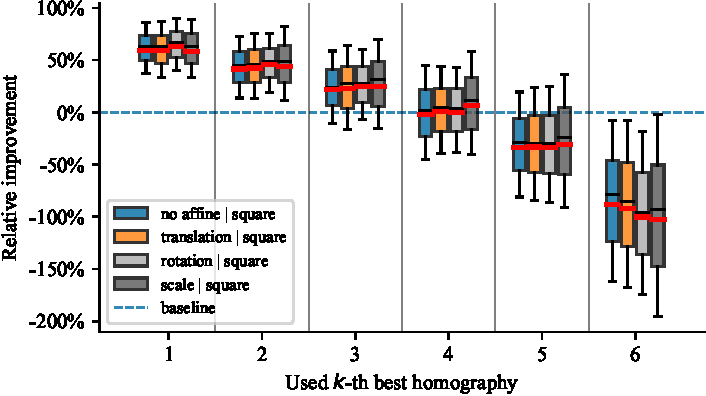
\includegraphics[width=\boxplotimgwidth]{figures/homography/similarity_transform_influence.pdf}
    \caption{Influence of similarity transformation on the reprojection error.}
    \label{fig:SimilarityTransformInfluence}
\end{figure}

\paragraph{Influence of Noise}
In Figure~\ref{fig:NoiseInfluence}, we can see the effect of noisy point correspondence that simulated inaccurate keypoint detection. The ranking method preserved the trend of the relative improvement in presence of noise. Absolute reprojection error demonstrated that unless noise was present, the errors varied on sub-pixel levels, so they were practically zero.

\begin{figure}[t]
    \centering
    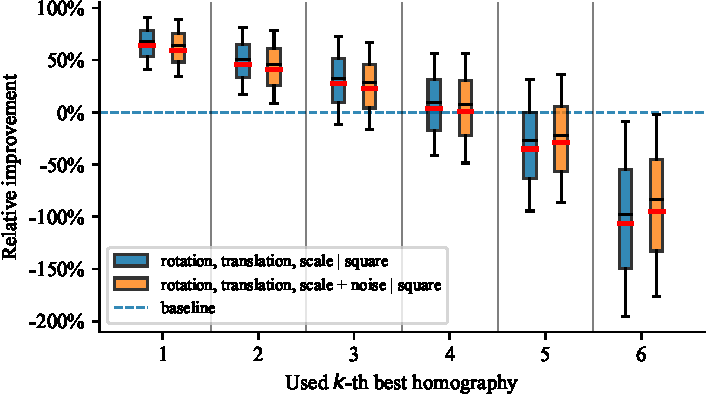
\includegraphics[width=\boxplotimgwidth]{figures/homography/noise_influence.pdf}
    \caption{Influence of noise applied to the warped keypoints representing a noisy point correspondence.}
    \label{fig:NoiseInfluence}
\end{figure}

\paragraph{Influence of Variable Shapes}
We expected that the relative improvement of our method should be invariant to variable shapes as long as they were similar. Figure~\ref{fig:ShapeInfluence} demonstrates that with an increasing number of keypoints our method consistently preserved its capabilities. Introducing more complicated shapes than just rectangles did not exacerbate the outcome of the algorithm.

\begin{figure}[t]
    \centering
    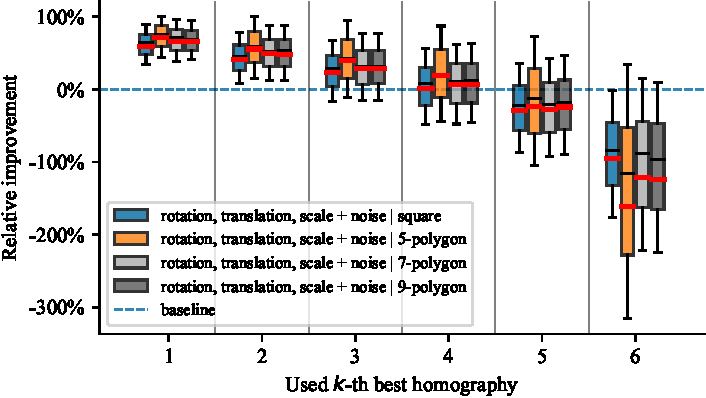
\includegraphics[width=\boxplotimgwidth]{figures/homography/shape_influence.pdf}
    \caption{Results for different marker shapes.}
    \label{fig:ShapeInfluence}
\end{figure}

\paragraph{Influence of Number of Markers}
We tested a variable number of markers to demonstrate that our method preserved its improvement. Figure~\ref{fig:NMarkersInfluence} shows that the greater the set of markers, the better the relative improvement of our method. Even when we used just three markers, the proposed method achieved a $46.91$\% median relative improvement.
While it is beneficial to use a larger number of markers, we believe that the improvement we can obtain from an increasing number of markers has a logarithmic trend. On the extreme side, if we used only one marker, there would be no improvement since there would be only one homography to choose from.

\begin{figure*}[t]
    \centering
    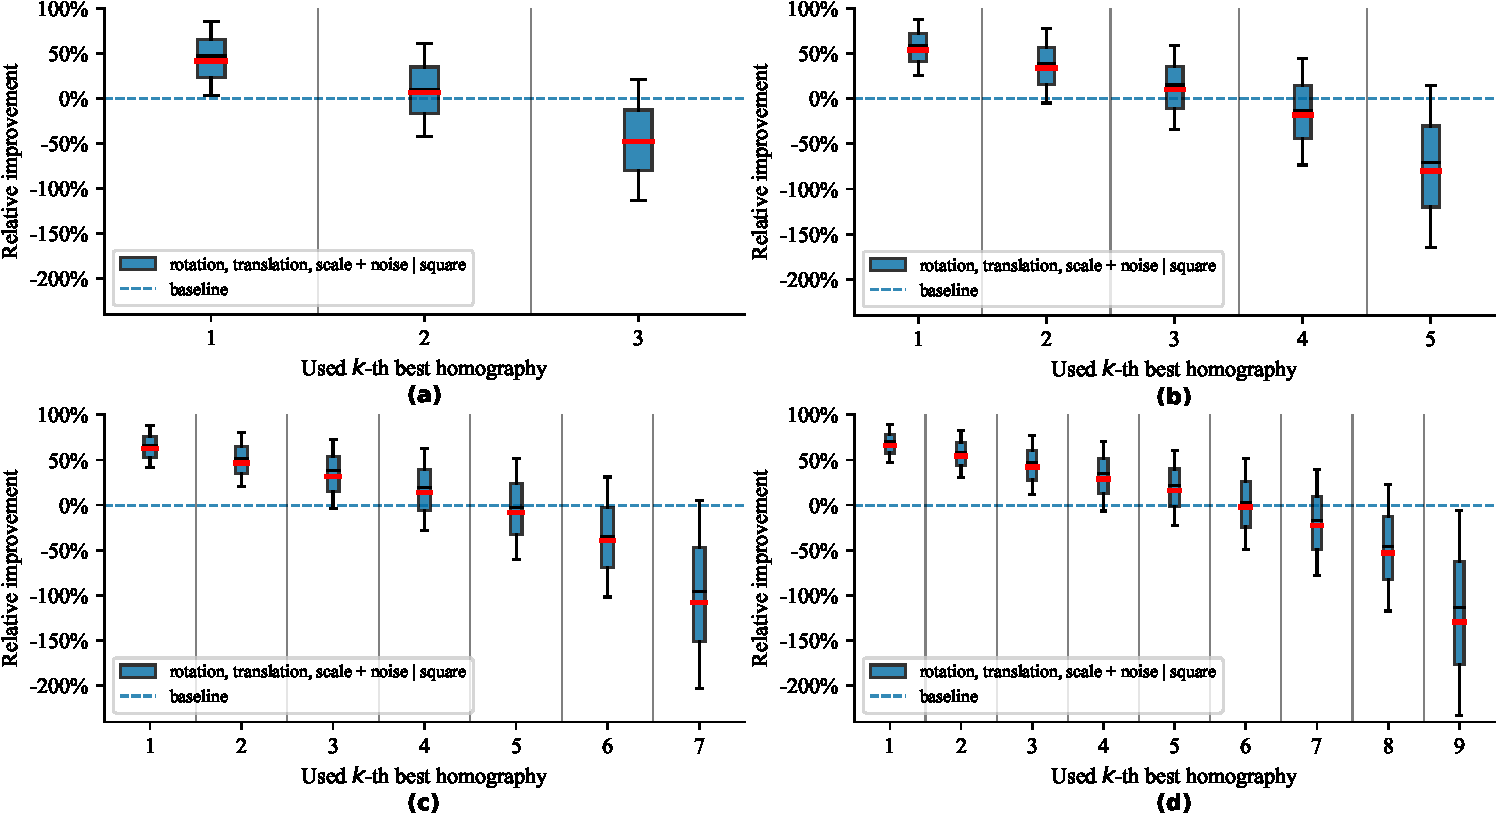
\includegraphics[width=\linewidth]{figures/homography/n_markers_influence.pdf}
    \caption{Influence of different number of markers on reprojection error. We experimented with \textbf{(a)} three, \textbf{(b)} five, \textbf{(c)} seven, and \textbf{(d)} nine markers.}
    \label{fig:NMarkersInfluence}
\end{figure*}

\def\tblsccolw{0.06}
\def\tblrscolw{0.08}
\begin{table*}[t]
    \caption{Description of test scenarios in our synthetic dataset with corresponding settings and results for the top-ranked homography. One row represents one test scenario. Four visually separated groups (from top to bottom) are related to experiments shown in Figure~\ref{fig:SimilarityTransformInfluence}~-~\ref{fig:NMarkersInfluence}.}
    \label{tab:TestScenariosResults}
    \setlength{\tabcolsep}{3pt}
    \begin{center}
        \footnotesize
        \begin{tabular}{p{\tblsccolw\linewidth}p{\tblsccolw\linewidth}p{\tblsccolw\linewidth}p{\tblsccolw\linewidth}p{\tblsccolw\linewidth}p{\tblsccolw\linewidth}|p{\tblrscolw\linewidth}p{\tblrscolw\linewidth}p{\tblrscolw\linewidth}p{\tblrscolw\linewidth}p{\tblrscolw\linewidth}p{\tblrscolw\linewidth}}
            \toprule
            \multirow{2}{2pt}{\textbf{shape}} &
            \multirow{2}{2pt}{\textbf{markers}} &
            \multirow{2}{2pt}{\textbf{transl.}} &
            \multirow{2}{2pt}{\textbf{rotation}} &
            \multirow{2}{2pt}{\textbf{scale}} &
            \multirow{2}{2pt}{\textbf{noise}} & \multicolumn{3}{l}{\textbf{top relative improvement}} & \multicolumn{3}{l}{\textbf{top absolute improvement}}\\
            & & & & & & \textbf{median} & \textbf{mean} & \textbf{stdev} &
            \textbf{median} & \textbf{mean} & \textbf{stdev}\\
            \midrule
            square &    6 &  no &  no &  no &  no & 62.80\% & 59.63\% & 19.64\% & 0.00029 & 0.00030 & 0.00014 \\
            square &    6 & yes &  no &  no &  no & 62.65\% & 59.00\% & 19.72\% & 0.00028 & 0.00029 & 0.00013 \\
            square &    6 &  no & yes &  no &  no & 66.42\% & 63.17\% & 19.11\% & 0.00041 & 0.00043 & 0.00020 \\
            square &    6 &  no &  no & yes &  no & 63.38\% & 58.51\% & 23.97\% & 0.00024 & 0.00025 & 0.00015 \\
            \midrule
            square &    6 & yes & yes & yes &  no & 67.82\% & 63.66\% & 20.30\% & 0.00035 & 0.00037 & 0.00019 \\
            square &    6 & yes & yes & yes & yes & 64.11\% & 59.26\% & 22.12\% & 22.07813 & 24.31773 & 15.00850 \\
            \midrule
            5-poly & 6 & yes & yes & yes & yes & 74.67\% & 71.19\% & 21.98\% & 69.55532 & 336.26534 & 685.74274 \\
            7-poly & 6 & yes & yes & yes & yes & 71.02\% & 65.63\% & 22.99\% & 46.79390 & 135.65737 & 395.75257 \\
            9-poly & 6 & yes & yes & yes & yes & 68.97\% & 65.57\% & 21.98\% & 44.97627 & 115.12189 & 309.27201 \\
            \midrule
            square &   3 &  yes & yes & yes & yes & 46.91\% & 41.36\% & 31.58\% & 14.77504 & 18.11548 & 20.67457 \\
            square &   5 &  yes & yes & yes & yes & 59.03\% & 53.91\% & 24.56\% & 19.76285 & 22.53333 & 16.00804 \\
            square &   7 &  yes & yes & yes & yes & 66.19\% & 62.41\% & 19.98\% & 23.87681 & 27.13637 & 32.28533 \\
            square &   9 &  yes & yes & yes & yes & 69.86\% & 66.09\% & 18.18\% & 25.66452 & 26.68378 & 11.69754 \\
            \bottomrule
        \end{tabular}
    \end{center}
\end{table*}
